%&<latex>
\documentclass[12pt]{exam}
\pagestyle{plain}
\usepackage{anysize}
\papersize{11in}{8.5in}
\marginsize{1in}{1in}{.5in}{.5in}
\pagenumbering{arabic}
\usepackage{setspace}
\usepackage[usenames]{color}
\usepackage[fleqn]{amsmath}
\usepackage{amssymb}
\usepackage{graphicx}
\usepackage{indentfirst}
\usepackage{ragged2e}
\usepackage{upgreek}
\usepackage{xspace}
\usepackage{ifthen}
\usepackage{parskip}
\usepackage[normalem]{ulem}
\usepackage[round]{natbib}
\bibliographystyle{evolution}
\usepackage{hyperref}
\hypersetup{pdfborder={0 0 0}, colorlinks=true, urlcolor=blue, linkcolor=blue, citecolor=blue}
\usepackage{enumitem}
\usepackage{tikz}
\usetikzlibrary{arrows}

\newcommand{\myIfArg}[2]{\ifthenelse{\equal{#1}{}}{}{#2}}

\providecommand{\e}[1]{\ensuremath{\times 10^{#1}}}
\newcommand{\ifTwoArgs}[3]{\ifthenelse{\equal{#1}{}\or\equal{#2}{}}{}{#3}\xspace}
\newcommand{\ifArg}[2]{\ifthenelse{\equal{#1}{}}{}{#2}\xspace}
\newcommand{\msb}{\upshape\texttt{msBayes}\xspace}
\newcommand{\meant}[2]{\ensuremath{E(\divt{#1})_{#2}}}
\newcommand{\vmratio}[1]{\ensuremath{\Omega_{#1}}}
\newcommand{\numt}[1]{\ensuremath{\Psi_{#1}}}
\newcommand{\divt}[1]{\ensuremath{\tau_{#1}}}
\newcommand{\ssVector}[1]{\ensuremath{\mathbf{\alignmentSS{#1}{}}}\xspace}
\newcommand{\ssVectorObs}{\ensuremath{\ssVector{}^*}\xspace}
\newcommand{\alignmentSS}[2]{\ensuremath{S_{#1\protect\ifTwoArgs{#1}{#2}{,}#2}}\xspace}
\newcommand{\ssMatrix}{\ensuremath{\mathbb \alignmentSS{}{}}\xspace}

\let\quoteOld\quote
\let\endquoteOld\endquote
\renewenvironment{quote}{\sffamily\slshape\small\quoteOld}{\endquoteOld}

\makeatletter
\renewcommand{\section}{\@startsection{section}{1}{0mm}%
    {-8pt}%
    {4pt}%
{\sffamily\large\itshape}}
\makeatother

\makeatletter
\newcommand*{\rom}[1]{\expandafter\@slowromancap\romannumeral #1@}
\makeatother

%% Basic formatting and spacing %%%%%%%%%%%%%%%%%%%%%
% \setlength{\parindent}{0em}
% \setlength{\parskip}{0.5em}

\tikzstyle{centered} = [align=center, text centered, font=\sffamily\bfseries]
\tikzstyle{skip} = [centered, inner sep=0pt, fill]
\tikzstyle{empty} = [centered, inner sep=0pt]
\tikzstyle{inode} = [centered, circle, minimum width=4pt, fill=black, inner sep=0pt]
\tikzstyle{tnode} = [centered, circle, inner sep=1pt]

\begin{document}
% \printanswers

\begin{center}
    \fbox{\parbox{5.5in}{\centering
            Please answer the following questions.
            Please {\bf DO NOT} provide your name.}}
\end{center}

\vspace{1cm}
\begin{questions}

\question I am an
\begin{oneparcheckboxes}
    \choice {\bf undergradute}
    \choice {\bf graduate}
\end{oneparcheckboxes}
student in year
\begin{oneparcheckboxes}
    \choice {\bf 1}
    \choice {\bf 2}
    \choice {\bf 3}
    \choice {\bf 4}
    \choice {\bf 5}
    \choice {\bf 6}
    \choice \rule[-0.5ex]{1cm}{0.5pt}
\end{oneparcheckboxes}
of my program of study.

\question Below are three rooted phylogenetic trees showing the
relationships of species A, B, C, and D. Which trees show the same
relationships?
\begin{checkboxes}
    \choice Tree \rom{1} and \rom{2}.
    \CorrectChoice Tree \rom{1} and \rom{3}.
    \choice Tree \rom{2} and \rom{3}.
    \choice All.
    \choice None.
\end{checkboxes}

\begin{center}
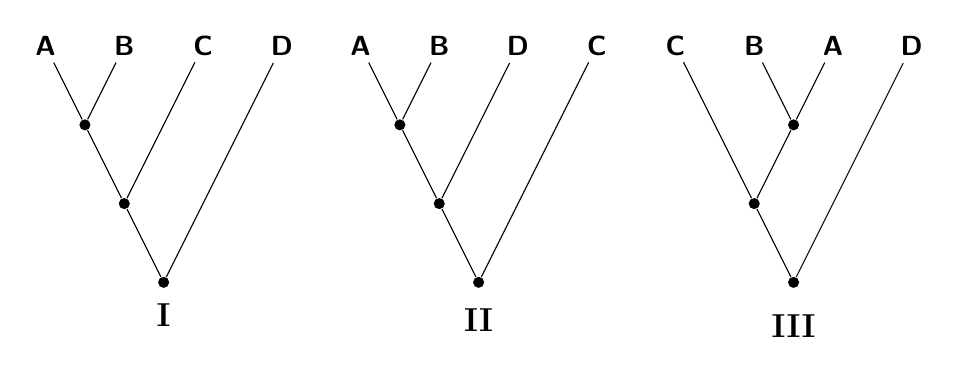
\begin{tikzpicture}
[scale=0.5,auto=left,every node/.style={circle}]%,fill=blue!20}]
  \node [tnode](a) at (1, 7) {A};
  \node [tnode](b) at (3, 7) {B};
  \node [tnode](c) at (5, 7) {C};
  \node [tnode](d) at (7, 7) {D};
  \node [inode](ab) at (2, 5)  {};
  \node [inode](abc) at (3, 3)  {};
  \node [inode, label=below: {\large\bf \rom{1}}](r) at (4, 1)  {};

  \foreach \from/\to in {r/abc,abc/c,abc/ab,ab/a,ab/b,r/d}
    \draw (\from) -- (\to);

  \node [tnode](a) at (9, 7) {A};
  \node [tnode](b) at (11, 7) {B};
  \node [tnode](c) at (13, 7) {D};
  \node [tnode](d) at (15, 7) {C};
  \node [inode](ab) at (10, 5)  {};
  \node [inode](abc) at (11, 3)  {};
  \node [inode, label=below: {\large\bf \rom{2}}](r) at (12, 1)  {};

  \foreach \from/\to in {r/abc,abc/c,abc/ab,ab/a,ab/b,r/d}
    \draw (\from) -- (\to);

  \node [tnode](c) at (17, 7) {C};
  \node [tnode](b) at (19, 7) {B};
  \node [tnode](a) at (21, 7) {A};
  \node [tnode](d) at (23, 7) {D};
  \node [inode](ab) at (20, 5)  {};
  \node [inode](abc) at (19, 3)  {};
  \node [inode, label=below: {\large\bf \rom{3}}](r) at  (20, 1)  {};

  \foreach \from/\to in {r/abc,abc/c,abc/ab,ab/a,ab/b,r/d}
    \draw (\from) -- (\to);

\end{tikzpicture}
\end{center}

\question In reference to the rooted Phylogeny \rom{4} below, which of the
following statements are correct?
\begin{checkboxes}
    \choice A and B are sister species.
    \choice Species B, C, and D are monophyletic.
    \choice Species A, B, and C are paraphyletic.
    \CorrectChoice Species D is more closely related to A than E.
\end{checkboxes}

\begin{center}
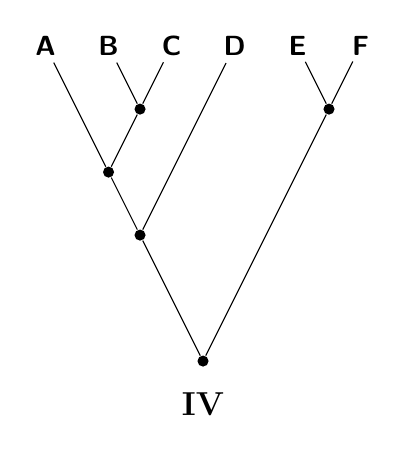
\begin{tikzpicture}
[scale=0.4,auto=left,every node/.style={circle}]%,fill=blue!20}]
  \node [tnode](a) at (1, 7) {A};
  \node [tnode](b) at (3, 7) {B};
  \node [tnode](c) at (5, 7) {C};
  \node [tnode](d) at (7, 7) {D};
  \node [tnode](e) at (9, 7) {E};
  \node [tnode](f) at (11, 7) {F};
  \node [inode](bc) at (4, 5)  {};
  \node [inode](ef) at (10, 5)  {};
  \node [inode](abc) at (3, 3)  {};
  \node [inode] (abcd) at (4, 1)  {};
  \node [inode, label=below: {\large\bf \rom{4}}](r) at (6, -3)  {};

  \foreach \from/\to in {bc/b,bc/c,abc/bc,abc/a,abcd/abc,abcd/d,r/abcd,r/ef,ef/e,ef/f}
    \draw (\from) -- (\to);

\end{tikzpicture}
\end{center}

\clearpage

\question In reference to the unrooted Phylogeny \rom{5} below, which of the
    following statements are always correct?
    \begin{checkboxes}
        \choice A and D are sister species.
        \choice Species A, D, and C are monophyletic.
        \choice Species D is more closely related to A than  B.
        \choice All of the above.
        \CorrectChoice None of the above.
    \end{checkboxes}

\begin{center}
\begin{tikzpicture}
[scale=0.55,auto=left,every node/.style={circle}]%,fill=blue!20}]
  \node [tnode](d) at (1,10.5) {D};
  \node [tnode](a) at (3,11) {A};
  \node [tnode](c) at (3,6) {C};
  \node [tnode](e) at (13,10) {E};
  \node [tnode](f) at (16,7) {F};
  \node [tnode](b) at (14,2) {B};
  \node [inode](ef) at (13,9) {};
  \node [inode](efb) at (12, 8) {};
  \node [inode](adc) at (4,7) {};
  \node [inode](ad) at (2, 10) {};
  \node [empty, label=above: {\large\bf \rom{5}}](l) at (8,6) {};

  \foreach \from/\to in {efb/ef,efb/b,adc/c,adc/efb,ad/a,ad/d,ad/adc,ef/e,ef/f}
    \draw (\from) -- (\to);

\end{tikzpicture}
\end{center}

\question Assuming the lengths of the branches on the unrooted Phylogeny
\rom{5} above are in units of evolutionary distance, what does the length of
each branch represent?
    \begin{checkboxes}
        \choice Time.
        \choice Rate of evolutionary change.
        \choice Geographic distance.
        \CorrectChoice The product of time and the rate of evolutionary change.
    \end{checkboxes}

\clearpage

\question Species A--F live along the side of a mountain. We notice that
individuals of species living at higher elevations tend to be larger than those
at lower elevations. We hypothesize that the species have adapted to grow
larger at higher elevations. We collect the following data on the adult
size and elevation of each species.

\begin{center}
\begin{tikzpicture}
[scale=0.55,auto=left,every node/.style={circle}]%,fill=blue!20}]
  \node [skip](xy) at (0,0) {};
  \node [empty](x) at (14,0) {};
  \node [empty](y) at (0,10) {};
  \node [empty, label=below: {\sffamily Elevation}](xl) at (7.5,0.5) {};
  \node [skip, label=left: {\sffamily Size}](yl) at (0,5) {};
  \node [inode, label=right: {\sffamily\bfseries A}](a) at (1,1) {};
  \node [inode, label=right: {\sffamily\bfseries B}](d) at (2.5,0.8) {};
  \node [inode, label=right: {\sffamily\bfseries C}](c) at (2,2.5) {};
  \node [inode, label=right: {\sffamily\bfseries D}](e) at (7,7.5) {};
  \node [inode, label=right: {\sffamily\bfseries E}](f) at (8.1,9.1) {};
  \node [inode, label=right: {\sffamily\bfseries F}](b) at (10,10) {};

  \foreach \from/\to in {xy/x,xy/y}
    \draw (\from) -- (\to);

\end{tikzpicture}
\end{center}

Below are two possible phylogenies for the species, one of which is correct.
Under which phylogeny are you more convinced that our hypothesis is correct?
    \begin{checkboxes}
        \choice \rom{6}
        \CorrectChoice \rom{7}
    \end{checkboxes}

\begin{center}
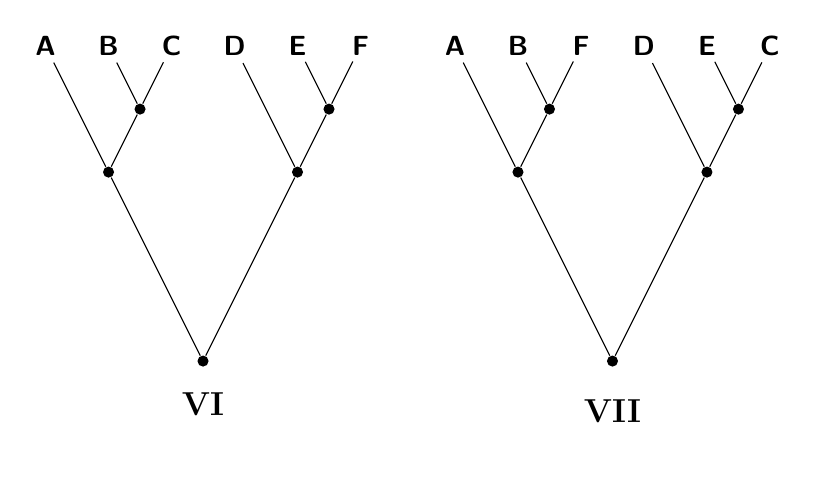
\begin{tikzpicture}
[scale=0.4,auto=left,every node/.style={circle}]%,fill=blue!20}]
  \node [tnode](a) at (1, 7) {A};
  \node [tnode](b) at (3, 7) {B};
  \node [tnode](c) at (5, 7) {C};
  \node [tnode](d) at (7, 7) {D};
  \node [tnode](e) at (9, 7) {E};
  \node [tnode](f) at (11, 7) {F};
  \node [inode](bc) at (4, 5)  {};
  \node [inode](ef) at (10, 5)  {};
  \node [inode](def) at (9, 3)  {};
  \node [inode](abc) at (3, 3)  {};
  \node [inode, label=below: {\large\bf \rom{6}}](r) at (6, -3)  {};

  \foreach \from/\to in {bc/b,bc/c,abc/bc,abc/a,r/abc,r/def,def/d,def/ef,ef/e,ef/f}
    \draw (\from) -- (\to);

  \node [tnode](a) at (14, 7) {A};
  \node [tnode](b) at (16, 7) {B};
  \node [tnode](c) at (18, 7) {F};
  \node [tnode](d) at (20, 7) {D};
  \node [tnode](e) at (22, 7) {E};
  \node [tnode](f) at (24, 7) {C};
  \node [inode](bc) at (17, 5)  {};
  \node [inode](ef) at (23, 5)  {};
  \node [inode](def) at (22, 3)  {};
  \node [inode](abc) at (16, 3)  {};
  \node [inode, label=below: {\large\bf \rom{7}}](r) at (19, -3)  {};

  \foreach \from/\to in {bc/b,bc/c,abc/bc,abc/a,r/abc,r/def,def/d,def/ef,ef/e,ef/f}
    \draw (\from) -- (\to);

\end{tikzpicture}
\end{center}

\end{questions}
\end{document}

